\documentclass{article}
\usepackage{graphicx} % Required for inserting images
\usepackage{amsmath}
\usepackage{float}


\title{Maze Game}
\author{N.K.Vishwaajith}
\date{April 2024}

\begin{document}

\maketitle
\tableofcontents
\newpage
\section{Introduction}
I believe all of us have played maze games at some point in our lives. I personally have played them a lot, usually in newspapers and magazines. The objective of the game is to navigate through a maze from the starting point to the ending point. The maze is a complex network of paths and walls, and the player must find the correct path to reach the end point while avoiding obstacles and traps. The game requires strategic thinking, problem-solving skills, and quick reflexes to complete each level successfully. \\
For this,  I have developed a maze game which involves a cat trying to reach from one stronghold to another, with time boosters and milk bottles(score boosters) which increase time and score respectively.\\
\section{Game Overview}
To start the game, you should write the following command in the terminal
\begin{center}
     python3 game.py 
\end{center}
This should trigger the raise of the main screen.\\ \\
\begin{figure}[H]
    \centering
    \includegraphics[width=0.75\textwidth]{Start_menu.png}
    \caption{Main screen}
    \label{fig:main_screen}
\end{figure}
Here we can see that there is an options button and buttons which lead to different levels.\\ \\
\begin{itemize}
    \item Level 1 : 20x20 grid to solve within 4 minutes
    \item Level 2 : 40x40 grid to solve within 4 minutes
    \item Level 3 : 60x60 grid to solve within 4 minutes
\end{itemize}
\\
The start point is always the top left corner and the goal is to reach the bottom right corner of the maze.\\
\begin{figure}[H]
    \centering
    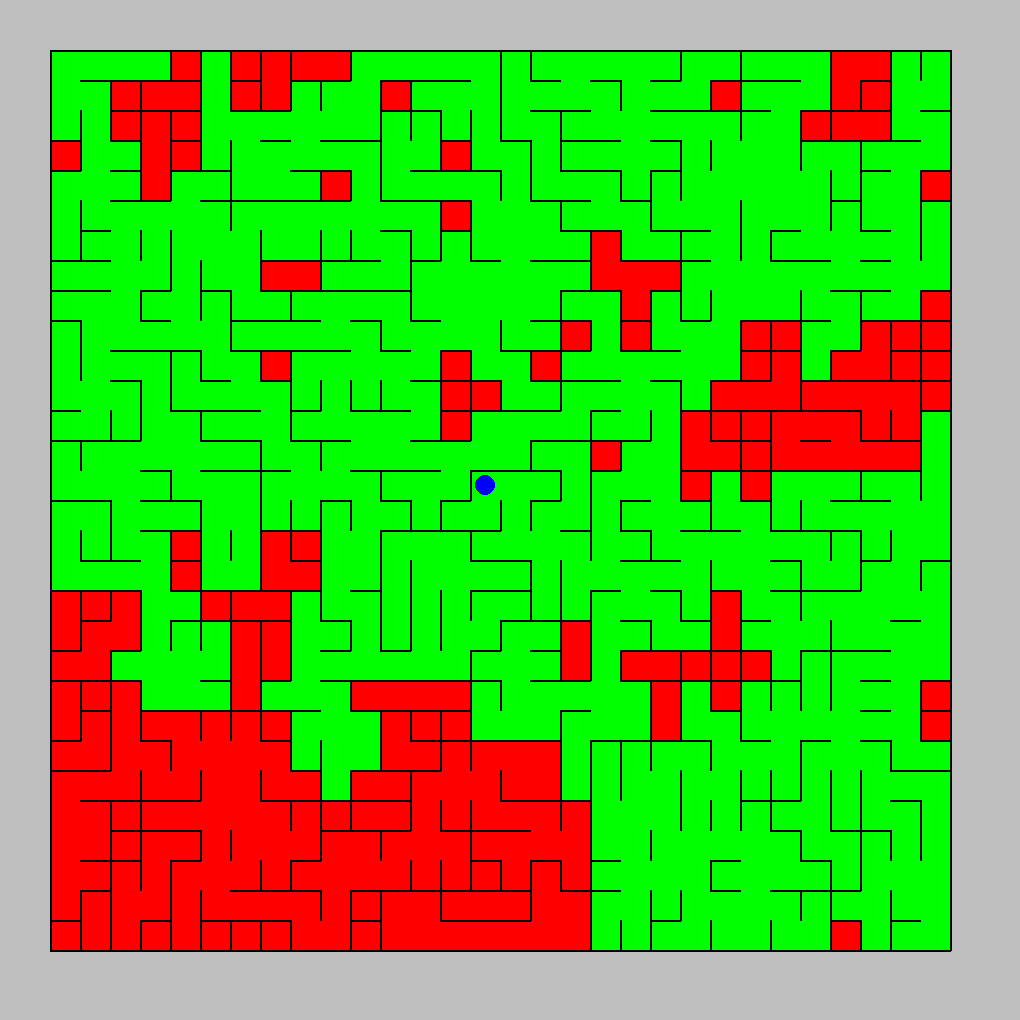
\includegraphics[width=0.75\textwidth]{maze.png}
    \caption{Game Start}
    \label{fig:Game_start}
\end{figure}
There are two sets of controls , which can be switched in the main menu by the options button, which leads you to the options menu where you can switch between two sets of controls by clicking the change controls button.
\begin{itemize}
    \item WASD controls:\begin{itemize}
        \item W : up
        \item A : left
        \item S : down
        \item D : right
    \end{itemize}
    \item Arrow controls:\begin{itemize}
        \item left arrow : left
        \item right arrow : right
        \item up arrow : up
        \item down arrow : down
    \end{itemize}
\end{itemize}
\begin{figure}[H]
    \centering
    \includegraphics[width = 0.75\textwidth]{options.png}
    \caption{option menu}
    \label{fig:option}
\end{figure}
Now, the game when selected a level,randomly generates a maze which has a single solution path from the start to the finish, which has collectibles in and around the path which u can use to boost your score and time.\\
The pink tiles are the tiles which we can move in and the blue tiles are tiles which we aren't allowed to move in. Attempting to go in to the blue tiles will bounce the cat back and put it back into the file.\\
If we want to exit the game midway, press space to go to the gameover screen which has a "Back to Main Menu" button.\\
\begin{figure}[H]
    \centering
    \includegraphics[width=0.75\textwidth]{gameover.png}
    \caption{Game over}
    \label{fig:game_over}
\end{figure}
The ending tile looks different and is visible easily, and once it is reached, the winscreen is shown and the cat goes into its resting animation with the score being displayed on top of it.\\
\begin{figure}[H]
    \centering
    \includegraphics[width=0.75\textwidth]{endtile.png}
    \caption{endtile}
    \label{fig:endtile}
\end{figure}
\begin{figure}[H]
    \centering
    \includegraphics[width=0.75\textwidth]{winscreen.png}
    \caption{Winscreen}
    \label{fig:winscreen}
\end{figure}
\section{Customizations}
There are 3 major customizations and other smaller customizations made in this game:
\begin{itemize}
    \item Sprite Animation
    \item Collectibles which increase the score
    \item intra cell movement
    \item options for different keybinds
    \item soothing background music
    \item Debug mode(cheats) which takes away collisions from walls
\end{itemize}
\subsection{Sprite Animation}
Each direction has its own set of animation frames which spans over 9 frames, and care has been taken to make it look smooth.\\
\subsection{Collectibles}
There are two different types of collectibles there:
\begin{itemize}
    \item 
\end{itemize}

\end{document}
